\chapter{Metodología experimental}
\label{chap:metodologia}

\section{Objetivo de la evaluación}
\label{sec:objetivo-evaluacion}

La evaluación experimental mide tres aspectos del comportamiento de OMP4Py sobre
los cinco benchmarks adaptados. Son la corrección, el rendimiento absoluto y
la escalabilidad. La corrección se comprueba mediante la verificación oficial de
cada benchmark. El rendimiento se mide con el tiempo interno reportado por NAS
y con los Mop/s de salida. La escalabilidad se estudia comparando el mejor
tiempo observado con 1, 2, 4, 8, 16 y 32~hilos dentro del mismo modo, clase e
intérprete. Como control de robustez, también se calcula la mediana y el rango
de las repeticiones válidas.

La comparación entre modos de ejecución articula el estudio. Los modos~0 y~1
sirven como referencia funcional y permiten cuantificar el coste de interpretar
directivas OMP4Py sin compilación. Los modos~2 y~3 son las configuraciones
orientadas a rendimiento, y la diferencia entre ambos mide el impacto del tipado
Cython sobre los kernels numéricos.


\section{Entorno de ejecución}
\label{sec:entorno-ejecucion}

Los experimentos se ejecutan en Finisterrae~III, el supercomputador del Centro
de Supercomputación de Galicia (CESGA), mediante el gestor de trabajos Slurm.
Se utilizan nodos de tipo \texttt{clk}, con procesadores Intel Xeon de 48 núcleos
y memoria DDR4. Las ejecuciones se limitan a 32~hilos para facilitar la
planificación de Slurm y cubrir los rangos de baja, media y alta concurrencia
dentro de un nodo.

El intérprete principal es Python~3.15.0b1t, compilado con soporte
\emph{free-threaded} (\texttt{--disable-gil}) en el directorio de usuario. Para
la comparación entre versiones se utilizaron también Python~3.13.13t y
Python~3.14.4t, ambos compilados como intérpretes \emph{free-threaded}. En las
tres versiones de la campaña comparativa se comprobó que el GIL estaba
desactivado.

Para aligerar tablas, figuras y análisis, el resto del documento usa las formas
abreviadas Python~3.13t, Python~3.14t y Python~3.15t. Estas abreviaturas se
refieren, respectivamente, a las compilaciones exactas Python~3.13.13t,
Python~3.14.4t y Python~3.15.0b1t descritas aquí.

El entorno de ejecución se automatiza mediante
\texttt{scripts/ft3/setup\_venvs.sh}, que crea un entorno virtual por versión
de Python e instala las dependencias necesarias. Las campañas finales usaron
NumPy~2.4.6 y Cython~3.2.5 en los tres intérpretes. El código fuente se mantuvo
idéntico entre versiones para que la variable experimental fuese el intérprete
y no la implementación del benchmark.

Las campañas finales no fijan por defecto variables de afinidad de OpenMP como
\texttt{OMP\_PROC\_BIND}, \texttt{OMP\_PLACES} o
\texttt{GOMP\_CPU\_AFFINITY}. Estas variables se eliminan explícitamente en los
scripts de ejecución salvo que se active un modo experimental específico. La
decisión evita que la política de afinidad del entorno distorsione la
comparación entre versiones y recuentos de hilos.


\section{Automatización de la campaña}
\label{sec:automatizacion-campana}

La ejecución en Finisterrae~III se automatiza con los scripts de
\texttt{scripts/ft3}. El script \texttt{make\_matrix.py} genera la matriz de
combinaciones de cada campaña, \texttt{submit\_campaign.sh} crea el directorio
de resultados y lanza el array de Slurm, \texttt{array\_run.sbatch} ejecuta los
trabajos, \texttt{run\_one.py} ejecuta una combinación concreta y
\texttt{parse\_results.py} reconstruye las tablas \texttt{summary.csv},
\texttt{summary\_best.csv} y los registros JSON. La
Figura~\ref{fig:metodologia-campana} resume este flujo.

\begin{figure}[htbp]
\centering
\resizebox{\textwidth}{!}{%
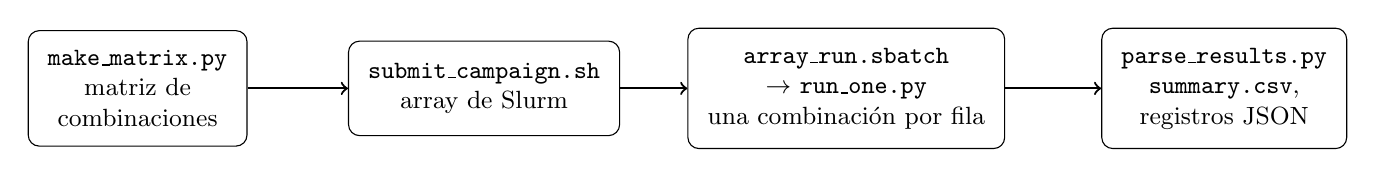
\begin{tikzpicture}[
  caja/.style={draw, rounded corners, align=center, minimum height=12mm,
               inner sep=2.5mm, font=\small},
  flecha/.style={->, thick}
]
  \node[caja] (matrix) at (0,0) {\texttt{make\_matrix.py}\\matriz de\\combinaciones};
  \node[caja] (submit) at (4.4,0) {\texttt{submit\_campaign.sh}\\array de Slurm};
  \node[caja] (run)    at (9.0,0) {\texttt{array\_run.sbatch}\\$\rightarrow$ \texttt{run\_one.py}\\una combinación por fila};
  \node[caja] (parse)  at (13.8,0) {\texttt{parse\_results.py}\\\texttt{summary.csv},\\registros JSON};
  \draw[flecha] (matrix) -- (submit);
  \draw[flecha] (submit) -- (run);
  \draw[flecha] (run) -- (parse);
\end{tikzpicture}
}
\caption{Flujo de la infraestructura de campaña en Finisterrae~III. Generación
de la matriz de combinaciones, envío como array de Slurm, ejecución de cada
combinación y consolidación de resultados.}
\label{fig:metodologia-campana}
\end{figure}

Cada fila de la matriz invoca el benchmark correspondiente mediante la
interfaz común descrita en el Capítulo~\ref{chap:adaptacion-nas}
(opciones \texttt{-c}, \texttt{-t} y \texttt{-m}).
Para cada ejecución se registra la salida estándar, la salida de error, el
código de retorno, el tiempo de proceso externo, el tiempo interno NAS, los
Mop/s y el estado de verificación. Las combinaciones se distribuyen entre
múltiples trabajos Slurm mediante arrays (\texttt{--array}), donde cada elemento
ejecuta varias filas de la matriz de forma secuencial. Esta organización
evita una ejecución monolítica, limita el número de trabajos enviados al
planificador y produce ficheros con nombres semánticos, no dependientes del
identificador interno de Slurm.

Una ejecución se considera válida si el proceso termina con código de retorno~0
y la verificación reporta \texttt{SUCCESSFUL}. Las ejecuciones con error, timeout
o verificación incorrecta se conservan en los resultados como indicadores de
limitaciones del modo o la implementación.


\section{Diseño de la matriz experimental}
\label{sec:matriz-experimental}

La evaluación se divide en dos bloques, una campaña principal con
Python~3.15.0b1t y una campaña comparativa entre versiones \emph{free-threaded}.

La campaña principal se divide en tres bloques por clase, y una campaña
comparativa añade la variación de intérprete. La
Tabla~\ref{tab:matriz-experimental} resume las cuatro configuraciones. Todas
ejecutan los cinco benchmarks (CG, EP, FT, IS, MG) con 1, 2, 4, 8, 16 y
32~hilos. Difieren en el intérprete, la clase, los modos evaluados y el número
de repeticiones.

\subsection{Campaña principal en clase S}
La clase~S es la más pequeña de las NAS y permite comparar los cuatro modos en
un tiempo razonable. Su papel principal es validar la corrección en todas las
combinaciones y cuantificar el coste relativo de cada modo con un único hilo.

\subsection{Campaña principal en clase W}
La clase~W es una carga de tamaño intermedio. Se restringe a los
modos~2 y~3 porque los modos~0 y~1 producen tiempos excesivamente altos en
cargas de este tamaño y no aportan información adicional sobre paralelismo real.

\subsection{Campaña principal en clase A}
La clase~A es la carga principal para analizar escalabilidad. En problemas de
mayor tamaño, el cociente entre trabajo útil y overhead de paralelización es más
favorable, por lo que esta campaña resulta más informativa. Se ejecuta
únicamente el modo~3 porque las clases~S y~W ya muestran que es el único modo
práctico para cargas grandes.

\subsection{Campaña comparativa entre versiones}
La campaña comparativa mantiene el mismo código fuente y ejecuta Python~3.13.13t,
Python~3.14.4t y Python~3.15.0b1t. Cubre las clases~S y~W. Los modos
compilados~2 y~3 se ejecutan en ambas clases, y los modos interpretados~0 y~1 se
añaden en clase~S, donde el código no compilado todavía termina en un tiempo
razonable y permite observar si la versión del intérprete influye en la
ejecución no compilada. La clase~S usa cinco repeticiones por combinación y la
clase~W usa tres.

\begin{table}[htbp]
\centering
\begin{tabular}{l|c|c|c|c}
 & \multicolumn{3}{c|}{Campaña principal} & Comparativa \\
\cline{2-4}
Parámetro & Clase S & Clase W & Clase A & versiones \\
\hline
Python & 3.15.0b1t & 3.15.0b1t & 3.15.0b1t & 3.13.13t, 3.14.4t, 3.15.0b1t \\
Clase & S & W & A & S, W \\
Modos & 0, 1, 2, 3 & 2, 3 & 3 & S (0--3), W (2, 3) \\
Repeticiones & 3 & 3 & 3 & S (5), W (3) \\
\end{tabular}
\caption{Matriz experimental. Todas las configuraciones ejecutan CG, EP, FT, IS
y MG con 1, 2, 4, 8, 16 y 32~hilos.}
\label{tab:matriz-experimental}
\end{table}

\subsection{Campaña de profiling}
Se lanzó una campaña específica de profiling con \texttt{perf stat}~\cite{LinuxPerfStat} para
relacionar los tiempos NAS con ocupación de CPU, IPC y eventos de memoria. Esta
campaña no repite toda la matriz experimental, sino que se concentra en los
casos necesarios para explicar por qué EP y FT escalan y por qué CG, IS y MG no
obtienen aceleración sostenida. Para evitar mezclar efectos de versión con el
diagnóstico de bajo nivel, el cuerpo de la memoria usa una matriz homogénea, con
los cinco benchmarks en clase~W, modo~3, con Python~3.15t y los recuentos de
1, 8 y 32~hilos. Los óptimos finos y la comparación entre versiones se analizan
en sus campañas correspondientes, y \texttt{perf stat} se usa aquí como apoyo
diagnóstico sobre la configuración principal.

\begin{center}
\small
\begin{tabular}{l|l}
Parámetro & Valores \\
\hline
Herramienta & \texttt{perf stat} \\
Benchmarks & CG, EP, FT, IS y MG \\
Python & 3.15.0b1t \\
Clase y modo & W, modo 3 \\
Hilos & 1, 8 y 32 \\
Métricas & CPUs utilizadas, ciclos, instrucciones, IPC y eventos de caché \\
\end{tabular}
\end{center}

Cada fila de profiling ejecuta primero una repetición de calentamiento y
después una repetición medida con \texttt{perf stat}. Esta separación reduce el
impacto de la compilación Cython en las métricas de rendimiento. Aun así, las
métricas de \texttt{perf stat} corresponden al proceso completo, no solo a la
ventana temporizada por NAS. En benchmarks muy cortos, como IS clase~W, esta
limitación obliga a interpretar los contadores como apoyo diagnóstico y no como
medida exacta del kernel.


\section{Justificación de la restricción de modos en clases grandes}
\label{sec:justificacion-modos}

Los modos~0 y~1 no incluyen compilación Cython. En clase~S, el modo~0 ya
multiplica los tiempos del modo~3 por factores que van de $16\times$ en FT a
$381\times$ en MG. Extender esos modos a clases W o~A consumiría
recursos de cluster desproporcionados sin añadir información relevante sobre la
escalabilidad paralela, que es el objetivo de las clases mayores. Por eso los
modos~0 y~1 se evalúan por completo solo en clase~S.

La misma lógica justifica no ejecutar modo~2 en clase~A dentro de la campaña
principal. El modo~2 es útil para cuantificar el efecto del tipado en clases~S
y~W, pero sus tiempos absolutos en W ya muestran que no es una configuración
práctica para cargas grandes. La comparación entre versiones se restringe a S y
W por el mismo motivo, ya que permite estudiar el efecto del intérprete sin multiplicar
el coste de la campaña con clase~A.


\section{Métricas y tratamiento de los resultados}
\label{sec:tratamiento-resultados}

La métrica principal es el tiempo NAS interno, es decir, el tiempo que el propio
benchmark mide entre el inicio y el fin del cómputo, excluyendo inicialización,
E/S y verificación. Los Mop/s reportados por el benchmark se utilizan como
métrica complementaria.

El análisis principal se basa en el mejor tiempo de las repeticiones válidas
para cada combinación. Esta elección es habitual en benchmarking de rendimiento,
porque aproxima el tiempo de ejecución menos perturbado por ruido del sistema y evita
que una interrupción puntual del nodo domine la comparación. Para que esa
decisión no dependa de una sola ejecución favorable, la campaña conserva todas
las repeticiones y calcula también mediana, coeficiente de variación y rango.

La Tabla~\ref{tab:resultados-estabilidad-repeticiones} resume esa estabilidad.
En la campaña principal, el coeficiente de variación mediano se mantiene entre
0.59\% y 0.75\% según la clase. En los modos compilados de la comparación entre
versiones queda en 0.61--0.64\%, y allí la diferencia mediana entre la mediana y
el mejor tiempo es inferior al 0.5\%. Los modos interpretados de esa comparación
son algo más variables, con un coeficiente de variación mediano del 1.59\% en
clase~S, debido sobre todo a EP y FT en ejecuciones largas no compiladas, aunque
la mediana se mantiene cerca del mejor tiempo. Por tanto, las conclusiones no dependen
de escoger una repetición aislada. La mediana conduce a la misma lectura, pero el
mejor tiempo se mantiene como referencia para calcular speedups y comparar
rendimiento.

\begin{table}[htbp]
\centering
\small
\adjustbox{max width=\textwidth}{%
\begin{tabular}{llrrrrrr}
\hline
Campaña & Clase & Comb. & Reps. & CV med. & CV p95 & Rango med. & Mediana/mejor med. \\
\hline
Principal & S & 117 & 351 & 0.67\% & 5.55\% & 1.52\% & 0.47\% \\
Principal & W & 60 & 180 & 0.59\% & 4.71\% & 1.27\% & 0.48\% \\
Principal & A & 30 & 90 & 0.75\% & 4.43\% & 1.66\% & 0.38\% \\
Versiones (comp.) & S & 172 & 860 & 0.64\% & 5.32\% & 1.65\% & 0.35\% \\
Versiones (comp.) & W & 180 & 540 & 0.61\% & 4.85\% & 1.37\% & 0.38\% \\
Versiones (interp.) & S & 180 & 900 & 1.59\% & 5.88\% & 4.16\% & 1.27\% \\
\hline
\end{tabular}}
\caption{Estabilidad de las repeticiones válidas. CV, rango y diferencia
mediana/mejor se calculan por combinación con mediana NAS mayor que cero.}
\label{tab:resultados-estabilidad-repeticiones}
\end{table}


Los casos con mediana NAS igual a 0.00~s se excluyen de los porcentajes relativos
de la tabla porque el cociente no está definido. Corresponden a ejecuciones muy
cortas de IS clase~S en modo~3, donde la resolución de dos decimales de la salida
NAS domina la medida. Esos casos sirven para confirmar corrección y orden de
magnitud, pero no para ratios finos.

La fórmula de speedup utilizada es

\begin{equation}
\mathrm{speedup}(t) =
  \frac{\mathrm{mejor\_tiempo}(1~\mathrm{hilo})}
       {\mathrm{mejor\_tiempo}(t~\mathrm{hilos})}
\end{equation}

El speedup se calcula siempre dentro del mismo modo y clase, de forma que el
denominador y el numerador comparten el mismo modo de ejecución. Un valor
inferior a~1 indica que la ejecución con más hilos fue más lenta que la
ejecución secuencial equivalente en ese modo. El límite superior alcanzable está
acotado por la fracción secuencial de cada benchmark, de acuerdo con la ley de
Amdahl~\cite{Amdahl1967}. Las reducciones, barreras y secciones críticas que no
se reparten entre hilos fijan el techo de escalabilidad de cada kernel.

Los resultados se clasifican en tres categorías. La primera comprende las
ejecuciones correctas y medibles. La segunda agrupa las ejecuciones correctas en
las que el overhead domina al trabajo útil. La tercera recoge las no viables, por
timeout, error o verificación incorrecta. Esta clasificación separa los límites
del algoritmo o del tamaño de clase de los fallos de implementación.


\section{Amenazas a la validez}
\label{sec:amenazas-validez}

La evaluación se diseñó para aislar el efecto del modo de ejecución, el número
de hilos y la versión del intérprete, pero conserva varias amenazas a la validez
que deben tenerse en cuenta al interpretar los resultados.

\subsection{Validez interna}
El ruido del cluster puede afectar ejecuciones individuales. Para mitigarlo, las
campañas usan repeticiones, conservan todos los registros y comparan el mejor
tiempo válido dentro de cada combinación. Esta decisión favorece la medida menos
perturbada por interferencias externas, y queda respaldada por la baja
variabilidad observada entre repeticiones. Además, las campañas finales eliminan
por defecto las variables de afinidad de OpenMP para evitar que una política de
pinning externa condicione la planificación de hilos del intérprete
\emph{free-threaded}.

\subsection{Validez de medida}
El tiempo principal es el tiempo interno NAS, no el tiempo total del proceso. Por
eso las conclusiones de rendimiento se refieren al kernel medido por cada
benchmark y no al coste de arranque, importación, compilación o verificación. En
benchmarks muy cortos, especialmente IS y MG en clase~S, la salida NAS con dos
decimales produce valores de 0.00~s o 0.01~s. Esos casos sirven para confirmar
corrección y tiempos absolutos bajos, pero no para calcular ratios finos. En el
profiling con \texttt{perf stat}, los contadores se recogen a nivel de proceso
completo. Por tanto, en ejecuciones de centésimas de segundo se usan como apoyo
diagnóstico y no como medida exacta del kernel.

\subsection{Validez externa}
Las campañas se ejecutan en nodos \texttt{clk} de Finisterrae~III y con un rango
máximo de 32~hilos. Los resultados caracterizan esa plataforma y ese rango de
concurrencia. Extrapolarlos a otros procesadores, políticas de afinidad o
recuentos de hilos requeriría repetir la campaña. La comparación entre versiones
se limita a las clases~S y~W por coste de cluster. La clase~A se mide con
Python~3.15t en la campaña principal, pero no se repite para Python~3.13t y
3.14t.

\subsection{Validez del instrumento}
El nuevo profiling de Python~3.15 se usa como diagnóstico complementario. La
campaña principal y la campaña de \texttt{perf stat} se ejecutan en
Finisterrae~III. El profiler de Python~3.15 también se ejecuta en
Finisterrae~III, en clase~S y modo~1, para que las primitivas Python del runtime
sean visibles al muestreo y al trazado. El trazado completó los cinco benchmarks
y proporciona recuentos exactos de regiones, hilos y barreras. El muestreo se
usa en los puntos que completaron de forma válida y aporta porcentajes de espera
en barreras y reducciones. Estas medidas no sustituyen a los tiempos de la
campaña principal, sino que se interpretan como evidencia estructural sobre
sincronización, creación de equipos y balance de carga.
